% !TEX root = ../notes.tex

% ================  Applied ML ==============

\section{Applied Machine Learning}

In this chapter, the pipeline of a {\emph{Machine Learning}} process is explained \footnote{A few interesting things can be read on GitHub repository of \href{https://github.com/papers-we-love/seattle/tree/master/useful-things-to-know-about-ml}{Paper-we-Love}}. Before discovering in-depth the ways which \emph{Machine Learning} can be applied, we summarize briefly, in Figure \ref{pic:time_usage}, the time usage of the \emph{ML} pipeline according to different approaches. 

\begin{figure}[H]%---------------FIG--------------
 \centering
 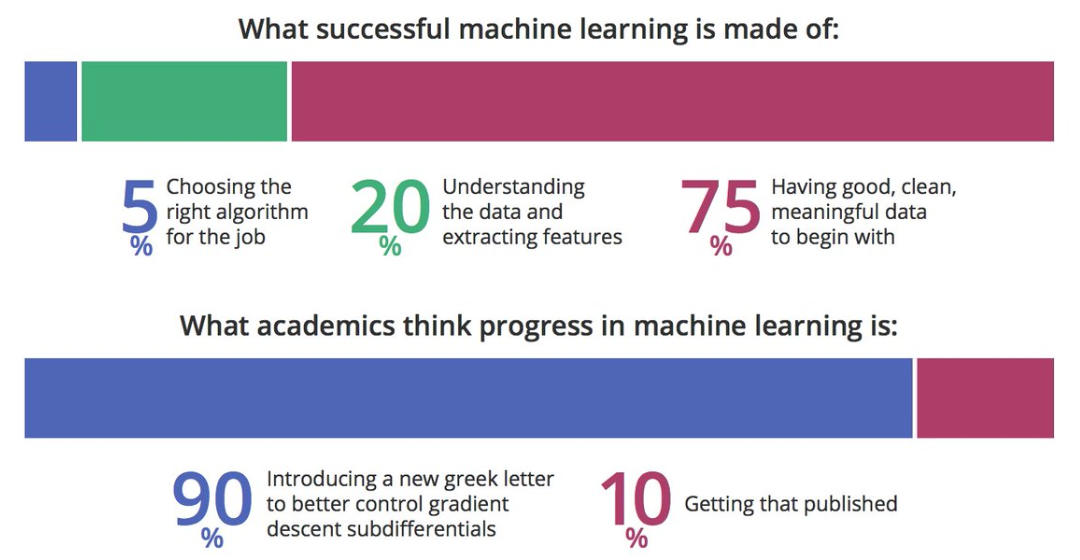
\includegraphics[width=13cm]{./img/08/time_usage}
 \caption{\label{pic:time_usage} Machine learning \emph{time usage}.}
\end{figure}

The showed pipeline refers to the \emph{Classification} problem, it can be generalized for regression though. The Figure \ref{pic:classification_pipeline}, clearly describes the main steps of the process.

\begin{figure}[H]%---------------FIG--------------
 \centering
 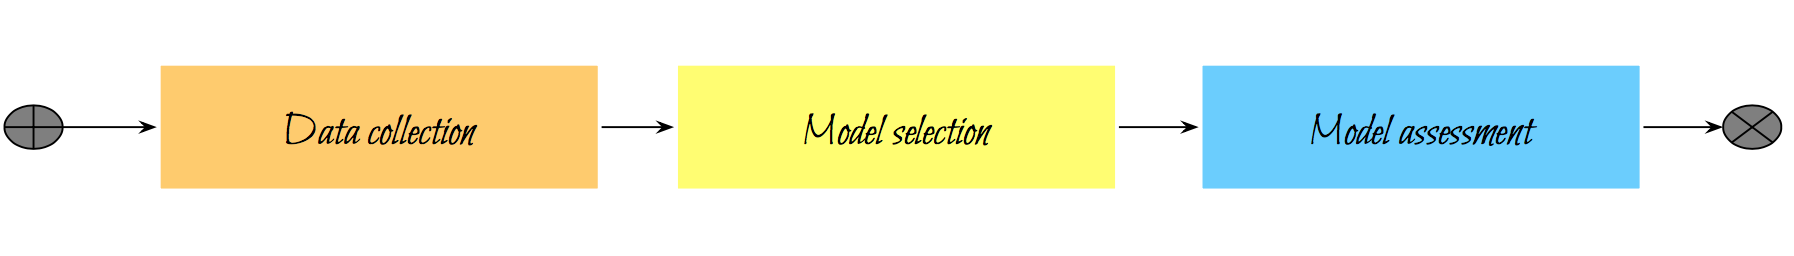
\includegraphics[width=13cm]{./img/08/classification_pipeline}
 \caption{\label{pic:classification_pipeline} Classification \emph{pipeline}.}
\end{figure}

\subsection{Data Collection}

The first step is the collection of data for a \emph{Classification} task. In particular, it consists in defining the \emph{attributes} that describe the data item of interest and the class label. In order to do that, a deep knowledge of the data domain is required. Furthermore, one of the most challenging aspects of the classification's \emph{data collection} is to get the class label for the items. In fact, most of the time the labels are missing. Trying to avoid and reduce this problem, many solutions have been proposed and most of them involve the interaction with humans. At this point be creative can be an extra-point, in fact you can use your imagination to try to figure out systems that allowed you to get the data.

In Figure \ref{pic:data_collection_pipeline}, we see more in-depth the pipeline of the \emph{Data Collection} step. 

\begin{figure}[H]%---------------FIG--------------
 \centering
 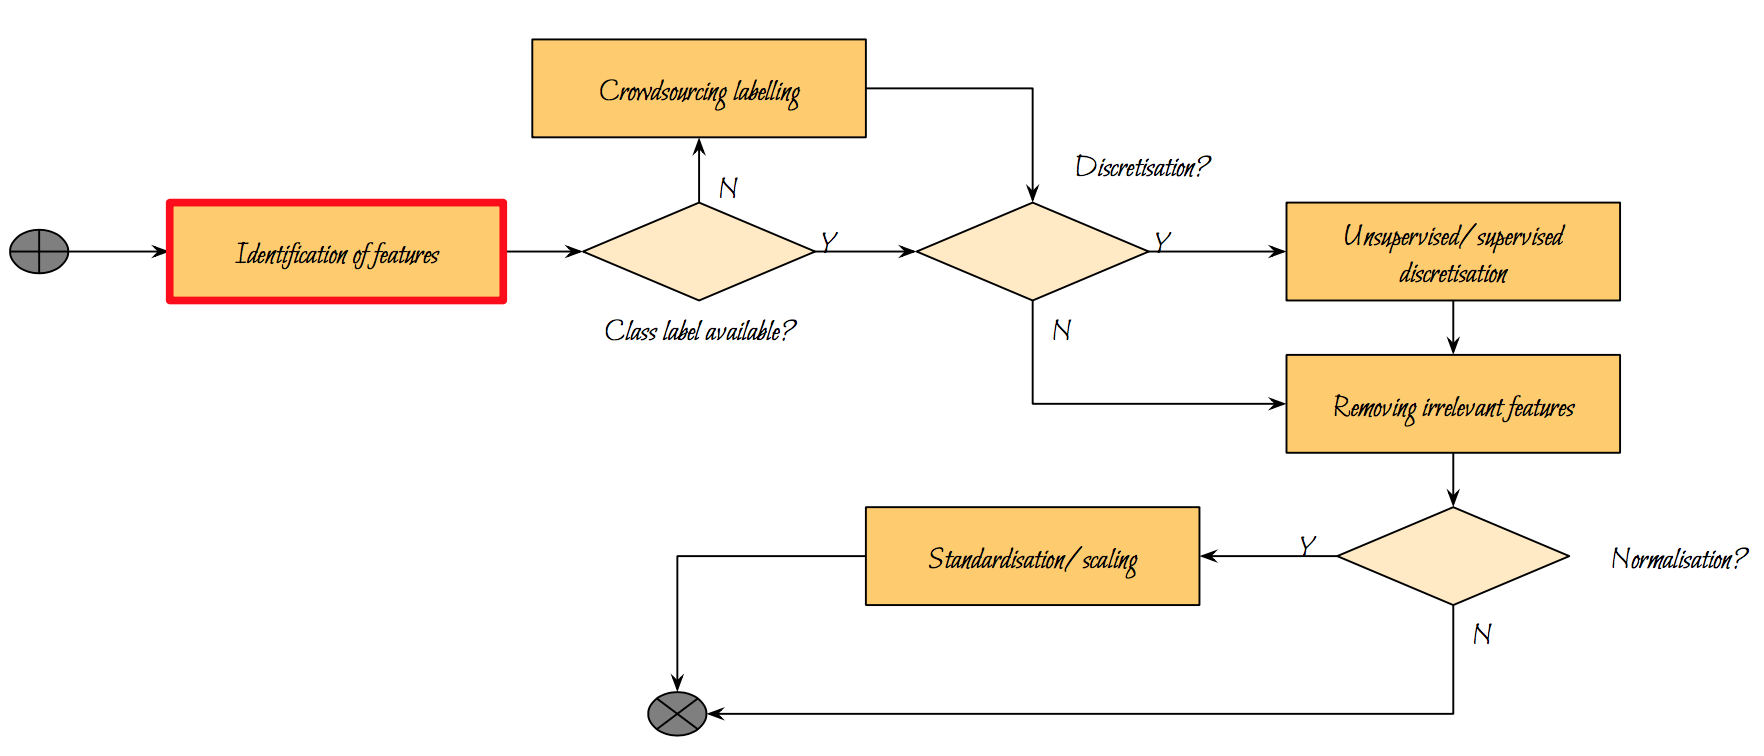
\includegraphics[width=13cm]{./img/08/data_collection_pipeline}
 \caption{\label{pic:data_collection_pipeline} Data collection \emph{pipeline}.}
\end{figure}

\subsubsection{Identification of features}

Since the feature describes the item we need to classify, their identification is a fundamental step in our pipeline. In particular we can distinguish between different types of features:
\begin{itemize}
\item \emph{Numerical} (e.g., age, temperature ...)
\item \emph{Ordinal} (e.g., phone code ...)
\item \emph{Categorical} (e.g., student, weather ...)
\end{itemize}

Moreover, new features can be generated from simple \emph{stats}, this process is known as \emph{Feature engineering} and  is considered a form of \emph{art}. It means that there are not specific rules to follow,  therefore the best suggestion is to look for people who have already attacked the same problem so that you can come up with new useful and powerful ideas.

Some classifiers, often, require categorical features. It implies that that the features should undergo a \emph{pre-processing} known as \emph{discretisation}. This procedure could be divided into two:
\begin{itemize}
\item \textbf{Unsupervised}: does not take class information into account
\begin{itemize}
\item \emph{Equal width}: divides the range into a predefined number of bins. The obvious weakness of the equal-width method is that in cases where the outcome observations are not distributed evenly, a large amount of important information can be lost after the discretisation process. 

\item \emph{Equal frequency}: divides the range into a predefined number of bins so that every interval contains the same number of values. For equal-frequency, many occurrences of a continuous value could cause the occurrences to be assigned into different bins. One improvement can be after continuous values are assigned into bins, boundaries of every pair of neighbouring bins are adjusted so that duplicate values should belong to one bin only.

\item \emph{Clustering}: The advantage of using clustering as discretisation is that it can be performed on all the features at the same time, capturing in this way possible interdependencies of the features. Sometimes discretisation can even improve the performance of algorithms that, theoretically, do not need it.
\end{itemize}

\item \textbf{Supervised}: takes class information into account, measuring the dependency of a discrete interval of values w.r.t. the class label as described below

\begin{itemize}
\item Test the hypothesis that two adjacent intervals of a feature are independent of the class 
\item If they are independent, they should be merged
\item Otherwise they should remain separate
\item Independence test: $\chi^2$ statistics
\end{itemize}
\end{itemize}

The feature \emph{pre-processing} and selection have changed over the year. Before 2012 (but still very common today) a clever design of the feature was considered the optimal recipe to make the model successful. After 2012 \footnote{Krizhevsky's publication on ImageNet classification is considered as a turning point: \href{https://papers.nips.cc/paper/4824-imagenet-classification-with-deep-convolutional-neural-networks.pdf}{Krizhevsky: ImageNet Classification with Deep Convolutional Neural Networks}}, 
the features and the model are learned together, in what is called mutually reinforcing.

\subsubsection{Data labeling}

Collecting lots of data is easy whereas labeling data is time consuming, difficult and sometimes even impossible. It is considered an extreme hard problem, moreover, based on subjective parameters. Nonetheless, there are ways to go beyond the limits of labeling, like the \emph{crowdsourcing}. The latter is, generally, represented by a platform where data is passed and the human label the interested item. There are many platforms for doing it (\href{https://en.wikipedia.org/wiki/CrowdFlower}{\emph{CrowdFlower}}, \href{https://www.clickworker.com}{\emph{ClickWorker}}, \href{https://en.wikipedia.org/wiki/Amazon_Mechanical_Turk}{\emph{MechanicalTurk}}).  Here, Figure \ref{pic:crowdsourcing}, an example, that shows the standard procedure of these platforms, follows . Consider we want to know whether a web page is or not reliable.  

\begin{figure}[H]%---------------FIG--------------
 \centering
 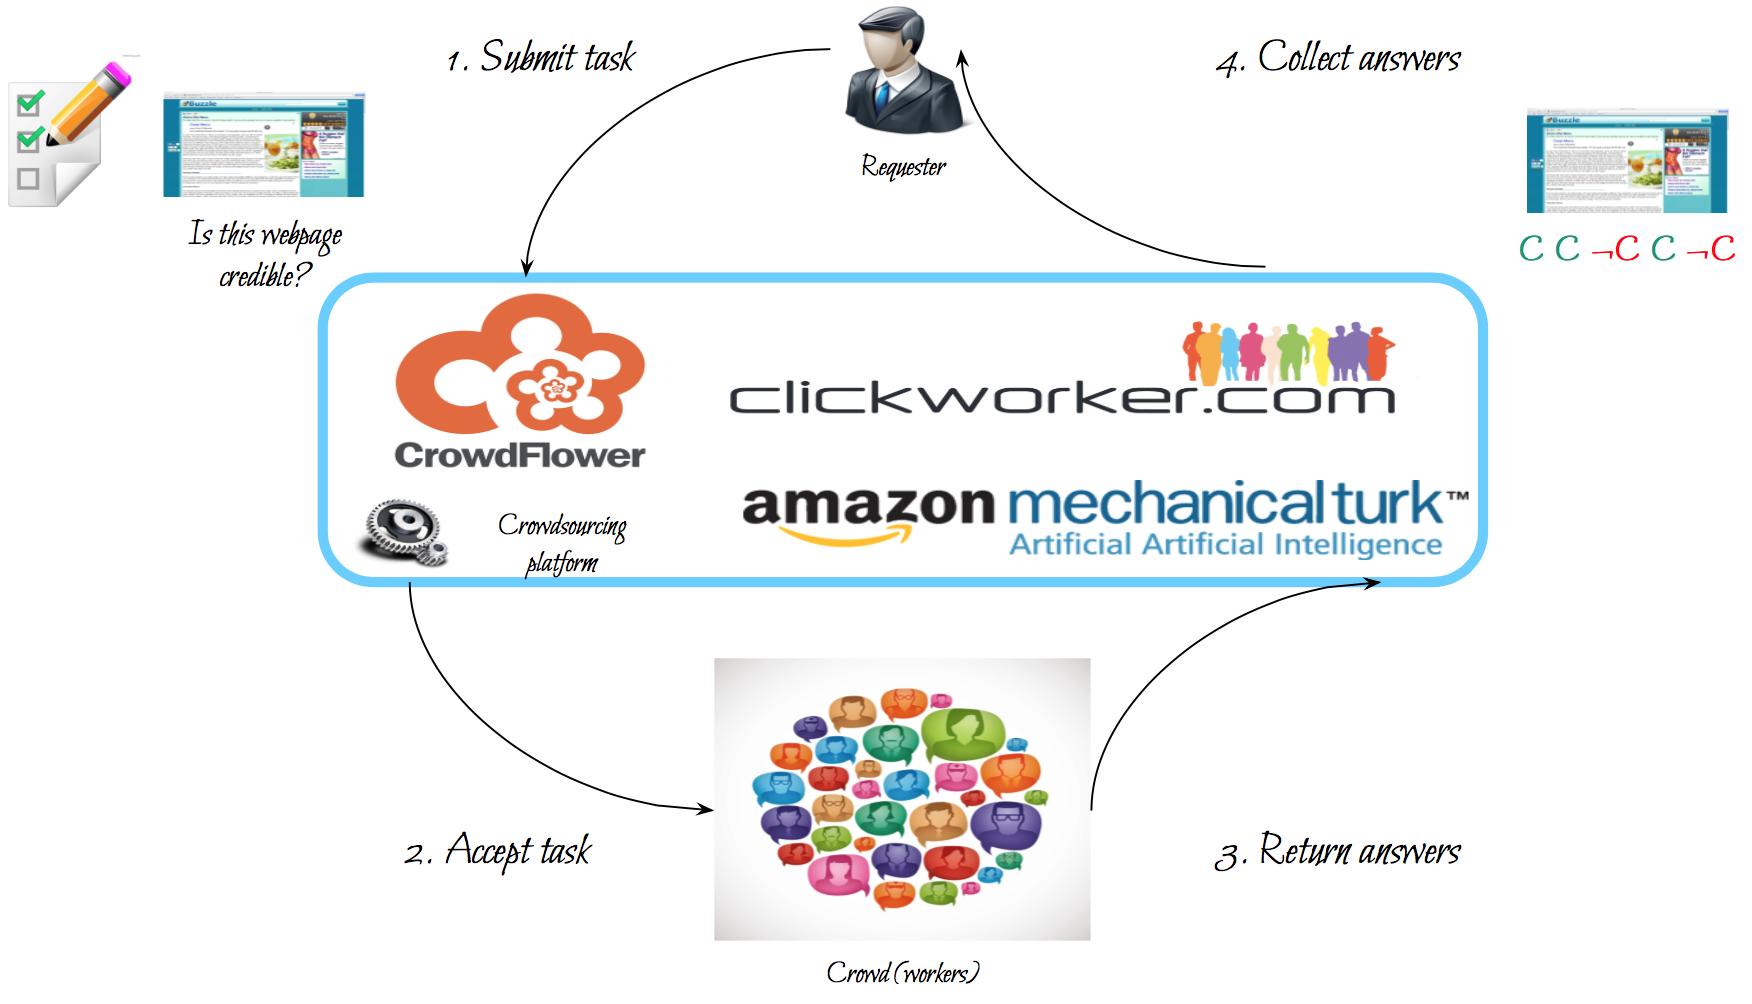
\includegraphics[width=13cm]{./img/08/crowdsourcing}
 \caption{\label{pic:crowdsourcing} \emph{Crowdsourcing} process.}
\end{figure}

You, the \emph{requester}, pass the data to the platform, once the task has been accepted the \emph{Crowd} (workers) return the answer. Before explaining how the answers are aggregated to finally label the item, it is important to consider the vast kinds of workers than can be faced.

\begin{center} %---------------TAB--------------
\begin{tabular} {| p{5 cm} | p{5 cm} |}
\hline
\bf Truthful & \bf Untruthful \\ \hline
+ \emph{Expert} & - \emph{Sloppy}: gives many wrong answers due to their knowledge limitations or misunderstanding  \\
+ \emph{Normal}  & - \emph{Uniform spammer}: gives random answers to any question \\
& - \emph{Random spammer}: keeps the same answer to every question \\
\hline
\end{tabular}
\end{center}


The Figure \ref{pic:worker_crowdsourcing}, shows how each type of worker tends to contribute to the \emph{true positive} and \emph{true negative}  rates.

\begin{figure}[H]%---------------FIG--------------
 \centering
 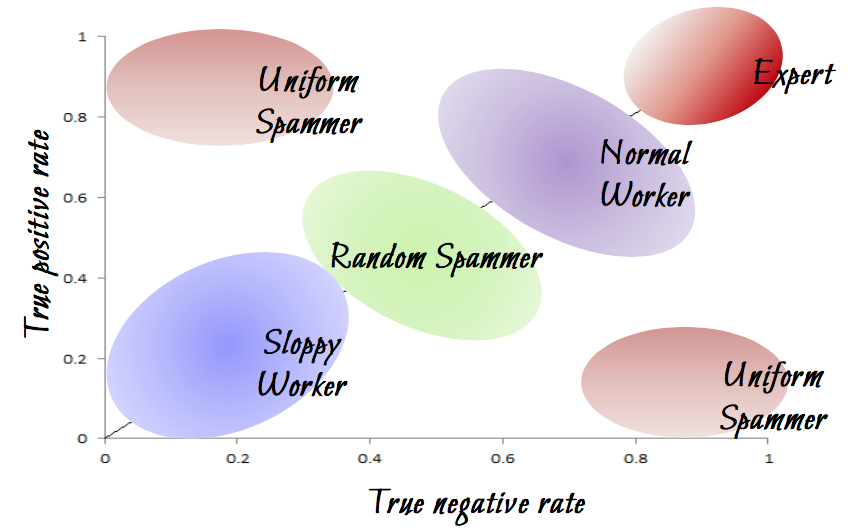
\includegraphics[width=13cm]{./img/08/worker_crowdsourcing}
 \caption{\label{pic:worker_crowdsourcing} \emph{Workers} outputs quality.}
\end{figure}

When the \emph{crowd} has labeled the item, so all the answers are collected, we proceed aggregating them. In particular, the label assigned to the item is the one that registers the highest number of occurrences, Figure \ref{pic:aggregation}.

\begin{figure}[H]%---------------FIG--------------
 \centering
 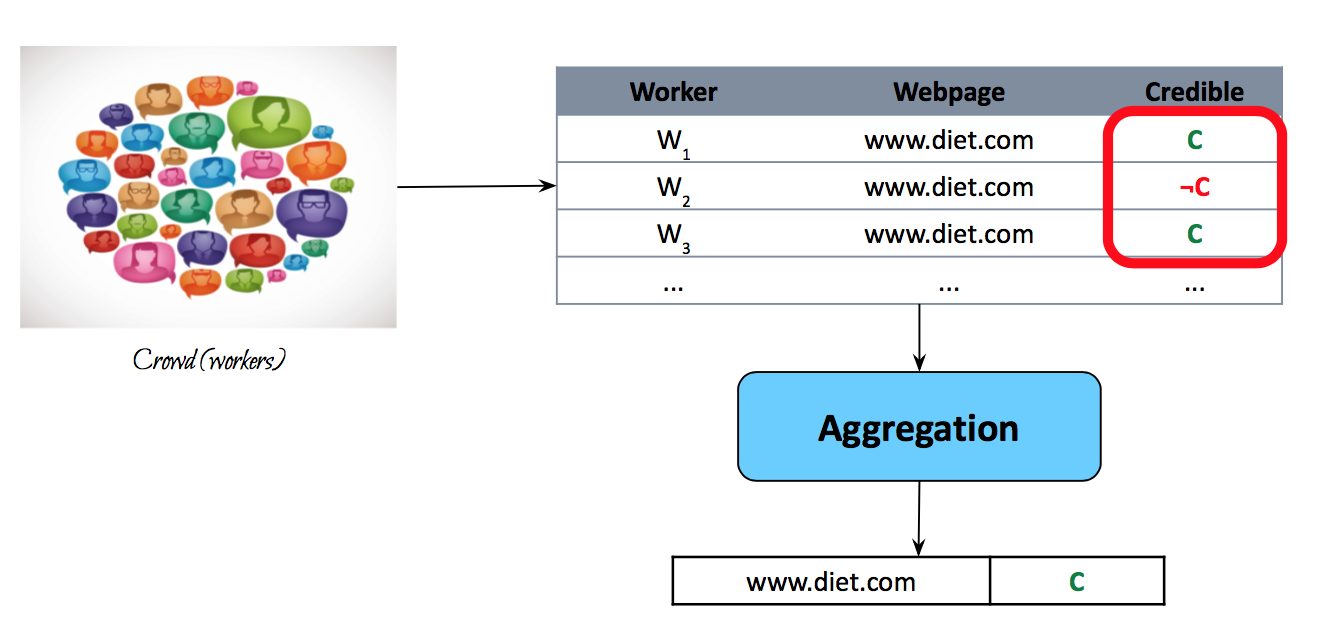
\includegraphics[width=13cm]{./img/08/aggregation}
 \caption{\label{pic:aggregation} Answer \emph{aggregation}.}
\end{figure}


\subsubsection{Feature Selection}

The aim of the \emph{Feature Selection} procedure is to reduce the number of \emph{N} features to a subset with the best $M < N$. The number of all the possible combination is $2^N$, when \emph{N} gets larger the required time to validate all the possible subsets of features sharply increases. Hence, there are two different available solution:
\begin{itemize}
\item \textbf{Filtering}: ranks features according to their predictive power and select the best ones
  \begin{itemize}
    \item[{\bf +}] Independent of the classifier (performed only once)
    \item[{\bf --}] Independent of the classifier (ignore interaction with the classifier)
    \item[{\bf --}] Assume features are independent
  \end{itemize}

  Defining $X$ as a feature and $Y$ as the class label. The ranking of the features is determined in different ways according to the kind of attribute:
  \begin{itemize}
    \item \textbf{Numerical}:
    \begin{itemize}
      \item \href{https://en.wikipedia.org/wiki/Pearson_product-moment_correlation_coefficient}{\emph{Pearson Correlation Coefficient}}
      $$\rho = \frac{\sum_{i=1}^{n}(X_i - \bar{X})(Y_i - \bar{Y})}{\sqrt{\sum_{i=1}^{n}(X_i - \bar{X})^2}\sqrt{\sum_{i=1}^{n}(Y_i - \bar{Y})^2}}$$

      \emph{Remark}: This metric only captures the linear relations! Furthermore, defining the correlation threshold is subjective (which is a good correlation value? 0.7 is enough?).

      \item \emph{Mutual information}: measures the information that $X$ and $Y$ share. In particular, it measures how much knowing one of these variables reduces uncertainty about the other. 

      $$ I(X,Y) = H(Y) - H(Y|X) = H(X) + H(Y) + H(X,Y)$$
      $$ H(X) = - \sum_{i}P(x_i)\log_2 P(x_i)$$
      $$ H(X,Y) = - \sum_{i}\sum_{j}P(x_i, y_j)\log_2 P(x_i, y_j)$$

      In particular,

      $$\left\{\begin{matrix}
      If \quad $I(X,Y) = 0$ & \quad X \quad does \quad not \quad tell \quad anything \quad about \quad Y\\ 
      Elif \quad $I(X,Y) = max$ & \quad X \quad tells \quad everything \quad about \quad Y
      \end{matrix}\right.$$
    \end{itemize}
    \item \textbf{Categorical}: 
    \begin{itemize}
      \item \href{https://en.wikipedia.org/wiki/Chi-squared_test}{$\chi^2$ method}: Different to correlation, the chi-square test checks the independence of the class and the feature, without indicating the strength or direction of any existing relationship. It is very powerful
    \end{itemize}
    A very important thing to keep in mind is that \textbf{collectively relevant features may look individually irrelevant!}. Hence, it is important to try to figure it out.
  \end{itemize}
  \item \textbf{Wrapper}: iteratively \textbf{adds} features, using cross-validation to guide feature inclusion and stopping when there is no improvement
  \begin{itemize}
    \item[{\bf +}] Interact with the classifier
    \item[{\bf +}] No independence assumption
    \item[{\bf --}] Computationally intensive
  \end{itemize}

  \item \textbf{Ablation}: iteratively \textbf{remove} features, using \emph{cross-validation} to guide feature inclusion and stopping when there is no improvement

  \begin{itemize}
    \item[{\bf +}] Interact with the classifier
    \item[{\bf +}] No independence assumption
    \item[{\bf --}] Computationally intensive
  \end{itemize}
\end{itemize}
  

\emph{Remark}: \href{http://www.tylervigen.com/spurious-correlations}{Beware of trusting} correlations in a blind way!! \emph{Correlation} is not \emph{causation}.

\subsubsection{Feature normalization}

Some classifiers do not manage well features with very different scales. Features with large values dominate the others, and most of the classifiers tend to capture and optimize the attribute that vary the most.

\begin{itemize}
\item \textbf{Standardization}: assumes that the data has been generated by a Gaussian process 
$$X_i' = \frac{(X_i - \mu_i)}{\sigma_i}$$
where $X_i$ is a feature, $\mu_i$ its mean and $\sigma_i$ its standard deviation. The new feature has $\mu_i = 0$ and $\sigma_i = 1$.

\item \textbf{Scaling}: if the data has outliers, they scale the \emph{normal} values to a very small interval

$$X_i' = \frac{(X_i - m_i)}{(M_i - m_i)}$$

where $X_i$ is a feature, $m_i$ its minimum and $M_i$ its maximum. The scaled belongs to the interval [0,1].

\end{itemize}

Before choosing the kind of normalization ti apply, we should understand what data we are using.

\subsection{Model selection}

\begin{figure}[H]%---------------FIG--------------
 \centering
 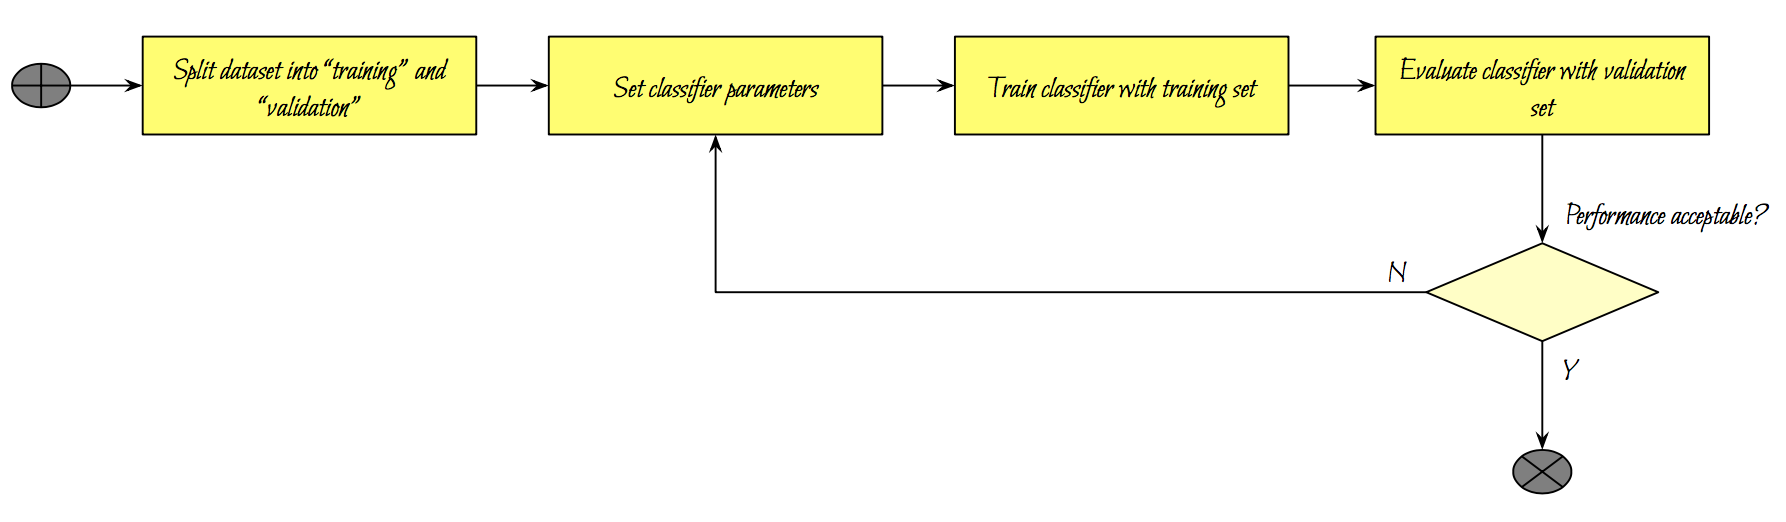
\includegraphics[width=13cm]{./img/08/model_selection}
 \caption{\label{pic:model_selection} Model selection \emph{pipeline}.}
\end{figure}

When we refer to the choice of a model, we do not only refer to the right classifier to pick but we also have to tune the parameters that characterize it. These parameters can be:
\begin{itemize}
\item \emph{Regularisation factor}: how complicated the model can grow (i.e. Ridge regression)
\item \emph{Threshold} 
\item \emph{Distance function} (i.e. KNN)
\item \emph{Number of neighbours} (i.e. KNN)
\end{itemize}

Moreover, it is necessary to define a metric that measures the performances of our model. We call the metric as \emph{Loss function}, and we distinguish between:
\begin{itemize}
\item \emph{Categorical output}
\begin{itemize}
\item \textbf{0-1 loss function}: counts how many labels are predicted correctly

$$J = \sum_{i=1}^{N} \#(y_i \neq f(x_i))$$
See section \ref{sec:perf} for more advanced cathegorical loss function.
\end{itemize}
\item \emph{Real value output}: 

\begin{itemize}
\item \textbf{Mean Squared Error (MSE)}
$$J = \frac{1}{n}\sum_{i=1}^{n} (y_i -  f(x_i))^2$$
\item \textbf{Mean Absolute Error (MAE)}
$$J = \frac{1}{n}\sum_{i=1}^{n} |y_i -  f(x_i)|$$
\end{itemize}

\end{itemize}

\begin{figure}[H]%---------------FIG--------------
 \centering
 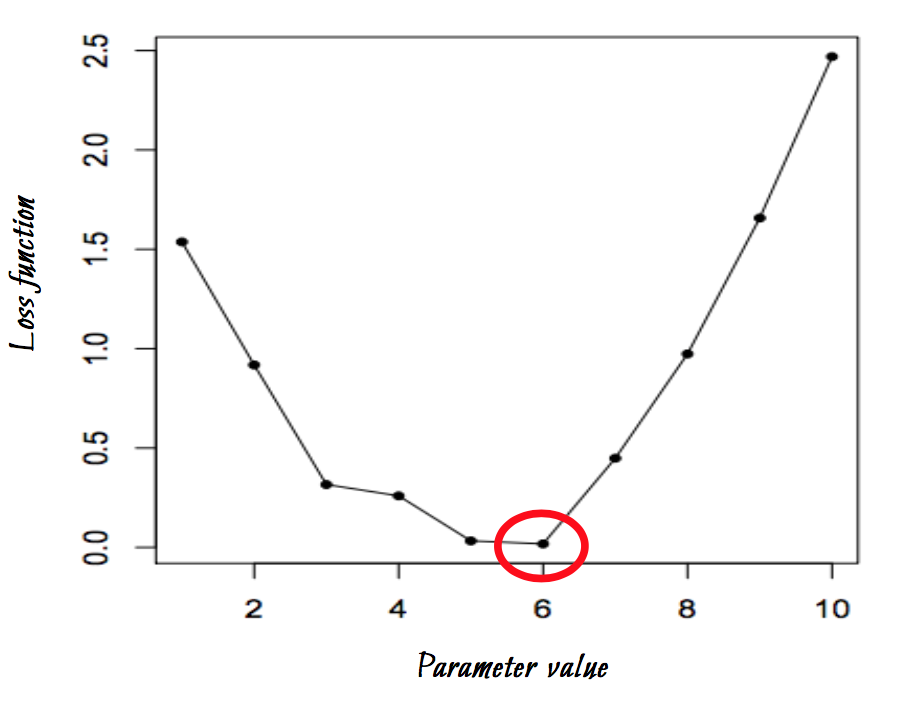
\includegraphics[width=13cm]{./img/08/loss_parameter}
 \caption{\label{pic:loss_parameter} Loss function as function of the parameter.}
\end{figure}

There are many other kinds of loss functions, \href{https://en.wikipedia.org/wiki/Loss_function}{look up} for them!

\subsubsection{More performance metrics for the binary classification}
\label{sec:perf}

For categorical binary classification, the usual metrics consider four types of errors, Figure \ref{pic:confusion_matrix}:

\begin{itemize}
\item \emph{True Positive}: positive examples classified as positive
\item \emph{True Negative}: negative examples classified as negative
\item \emph{False Positive}: negative examples classified as positive
\item \emph{False Negative}: positive examples classified as negative
\end{itemize}

\begin{figure}[H]%---------------FIG--------------
 \centering
 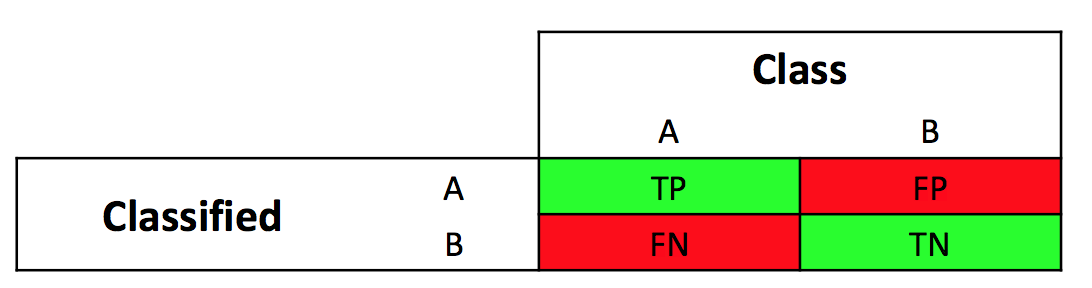
\includegraphics[width=13cm]{./img/08/confusion_matrix}
 \caption{\label{pic:confusion_matrix} Confusion matrix.}
\end{figure}

According to what we want to control with our model we want to choose the most appropriate metric:
\begin{itemize}
\item \textbf{Accuracy}: generally used when the classes are not skewed
and the errors have the same importance

$$A = \frac{TP+TN}{TP+TN+FP+FN} =  \frac{TP+TN}{N}$$

\item \textbf{Precision}: 
$$P = \frac{TP}{TP+FP}$$

High precision means that few irrelevant examples treated as important 
\item \textbf{Recall}: 
$$	R = \frac{TP}{TP+FN}$$
High recall means that that the classifier is good at getting the positive class right
\end{itemize}

Let's see an example, Figure \ref{pic:example}:

\begin{figure}[H]%---------------FIG--------------
 \centering
 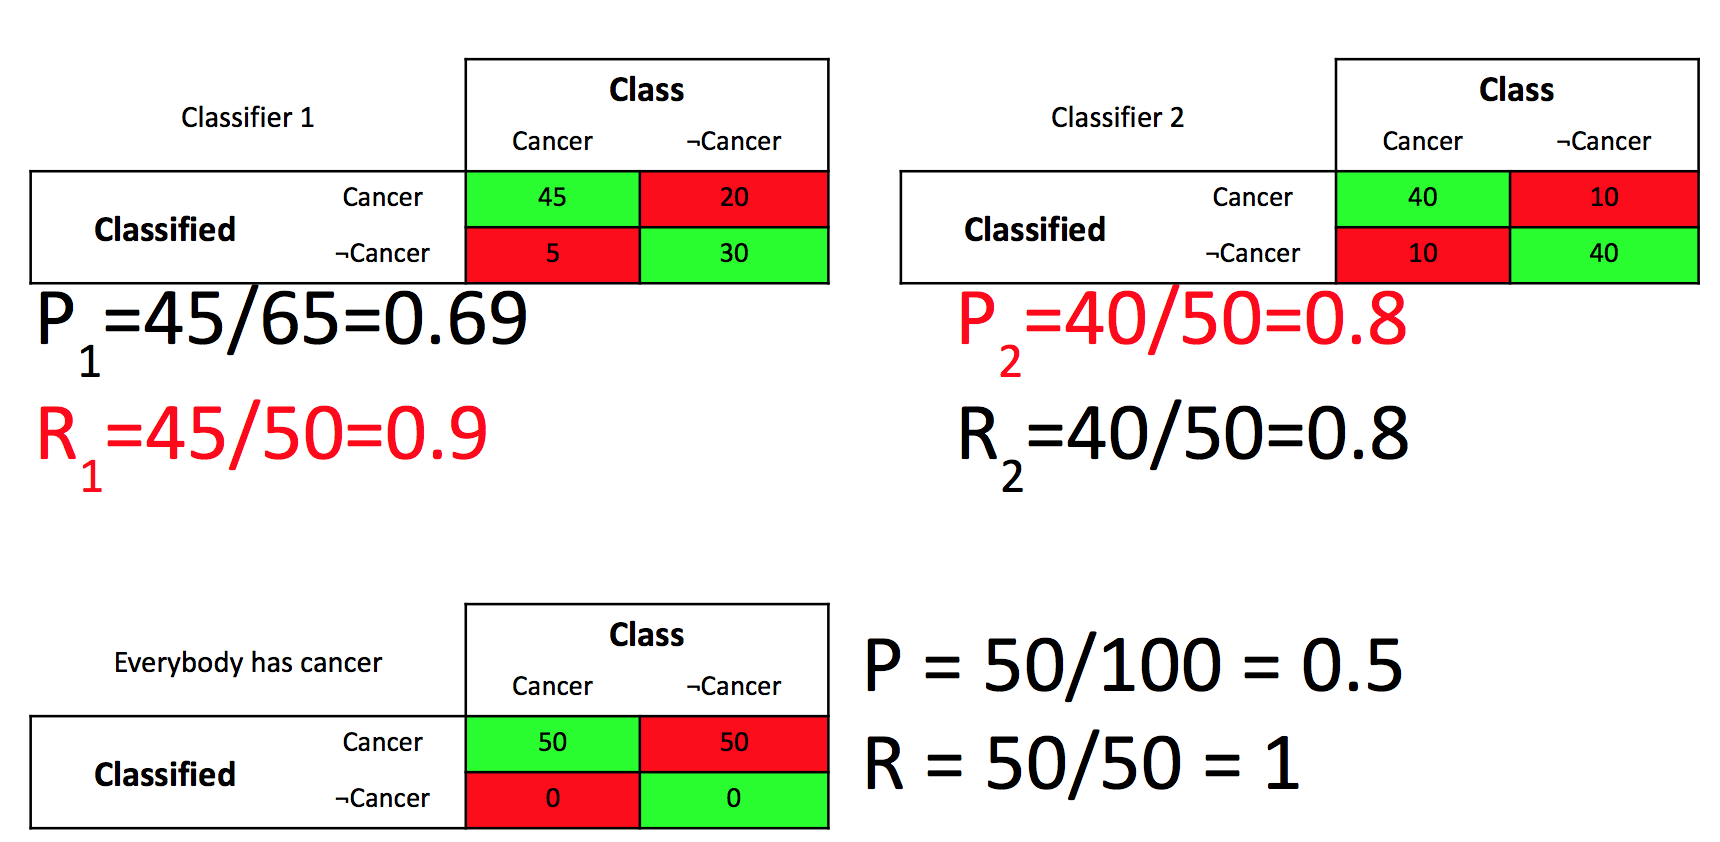
\includegraphics[width=13cm]{./img/08/example}
 \caption{\label{pic:example} Example.}
\end{figure}

We see that the classifier 2 is more precise at hitting the cancer, in fact few patients erroneously diagnosed with cancer. Classifier 1 has a better recall, few patients with cancer are not diagnosed correctly. 
The classifier "Everybody Has Cancer" detects all the patients with cancer, but also causes that 50\% of the patients with no cancer go home worried about their health status.

Due to the fact that to compare different classifiers we need a unique metric, we introduce

\begin{itemize}
\item \textbf{F-Score}: 

$$F = 2 \cdot \frac{w_p P \cdot w_r R}{P + R}$$
\end{itemize}

That is the harmonic average of the \emph{Precision} and the \emph{Recall}. Whether one is more important than the other  they can be differently weighted by setting $w_p$ and $w_r$.


For a graphical vision we introduce the \href{https://en.wikipedia.org/wiki/Receiver_operating_characteristic}{ROC \emph{Area Under the Curve}}, a single number that captures the overall quality of the classifier. It should be between 0.5 (random classifier) and 1.0 (perfect classifier). 

\begin{figure}[H]%---------------FIG--------------
 \centering
 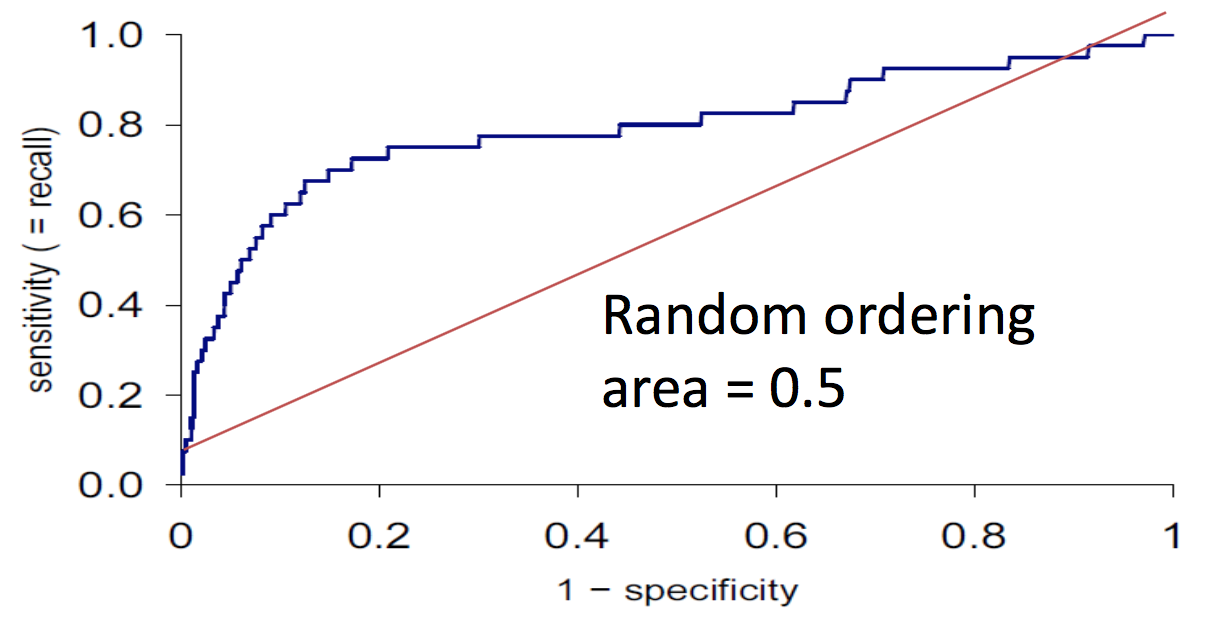
\includegraphics[width=13cm]{./img/08/roc}
 \caption{\label{pic:roc} ROC AUC. \emph{Y-axis}: true positive rate = $\frac{TP}{(TP + FN)}$, same as recall, \emph{X-axis}: false positive rate =$\frac{FP}{(FP + TN)} =$ 1 - specificity.}
\end{figure}

Since we have presented some usable metrics to verify the power of the model, we proceed to describe the pipeline used for the model selection.

\subsubsection{Split data into Training and test set}

Out inter set of data is split into two parts, generally, 60\% training set and 40\% test set. The former is used to learn the model, once it has been found it is evaluated, according to the chosen metric, on the test set. Take a look at Figure \ref{pic:train_test}.

\begin{figure}[H]%---------------FIG--------------
 \centering
 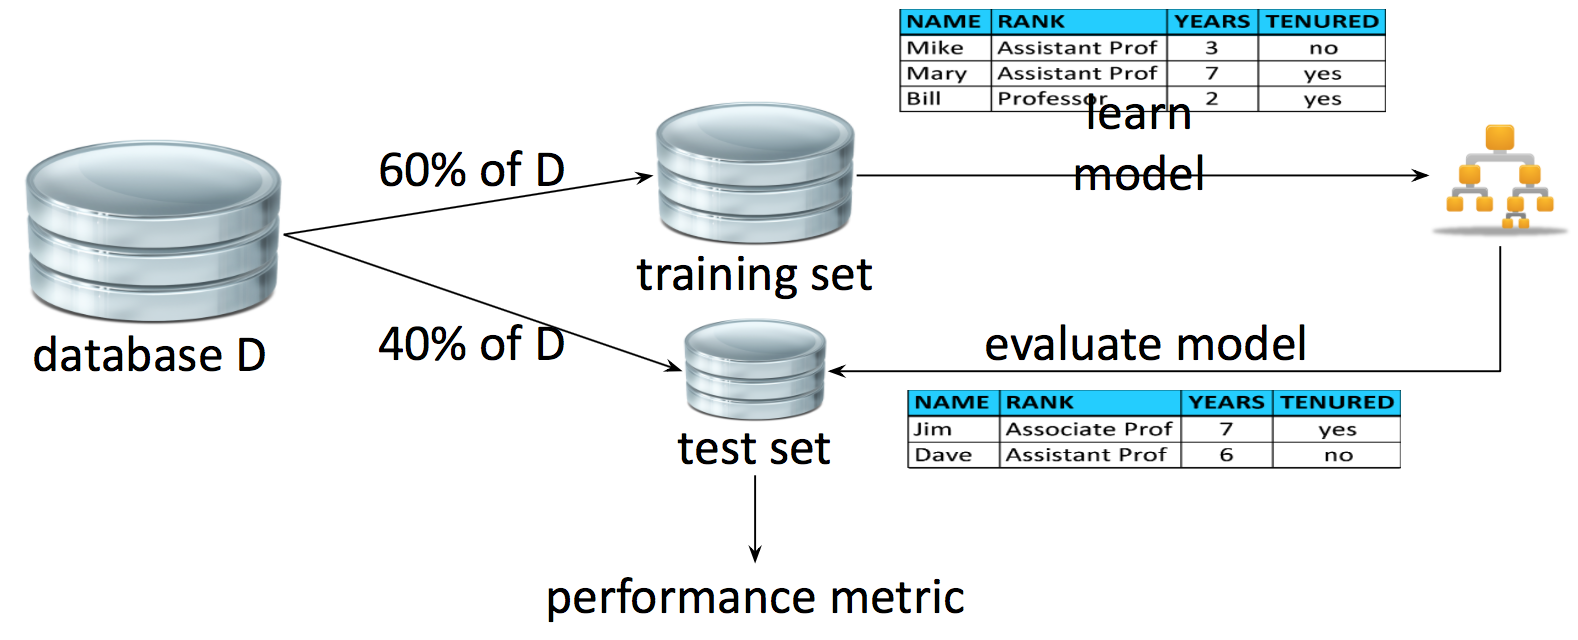
\includegraphics[width=13cm]{./img/08/train_test}
 \caption{\label{pic:train_test} \emph{Train} and \emph{test}.}
\end{figure}

\subsubsection{Tune parameters through the Cross-Validation and Bias Variance trade-off}

We present two different types of \emph{Cross-Validation}:
\begin{itemize}
\item \emph{Leave-One-Out Cross-Validation (LOO)}: which train the model on all the data except one sample which the model is tested on. This operation is repeated for each sample, Figure \ref{pic:loo}. This form of \emph{CV}  is almost unbiased (=not optimistic) estimate of the true accuracy, however, is time consuming because it performs a number of iterations equal to the number of samples in the data set. The evaluation of the model is the average of the errors obtained after each iteration.

\begin{figure}[H]%---------------FIG--------------
 \centering
 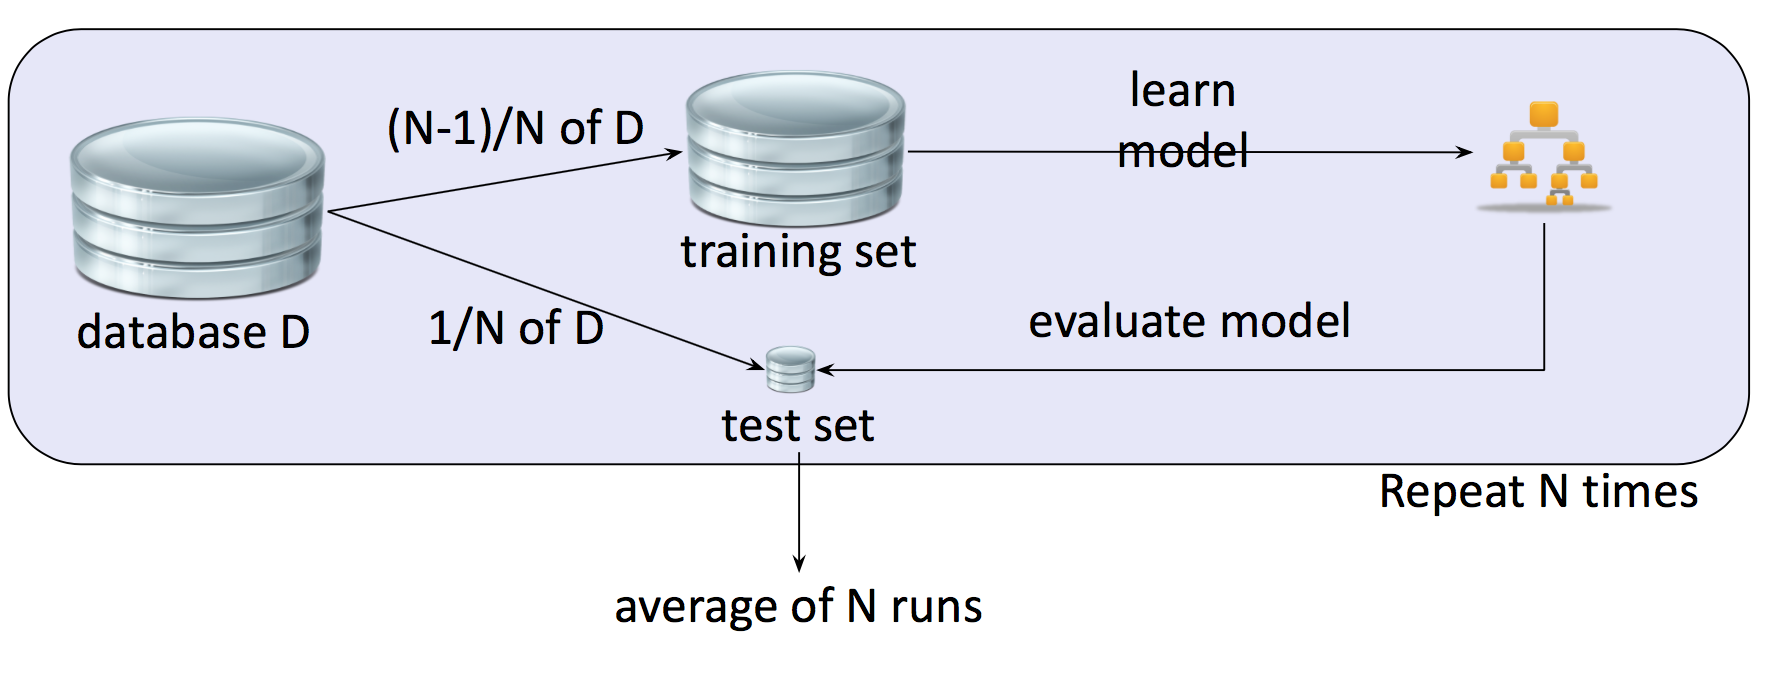
\includegraphics[width=13cm]{./img/08/loo}
 \caption{\label{pic:loo} \emph{LOO} cross validation.}
\end{figure}

\item \emph{K-Fold Cross-Validation}: which splits the data into K folds of equal size, Figure \ref{pic:kfold}. In turn, $K-1$ folders are used as train set and the remaining as test. Also in this case, the evaluation of the model is defined as the average of the errors obtained after all the iterations. This kind of \emph{CV} is a good compromise between having an unbiased estimate of the true accuracy and computation time. The most widely used $K$ number is 10.

\begin{figure}[H]%---------------FIG--------------
 \centering
 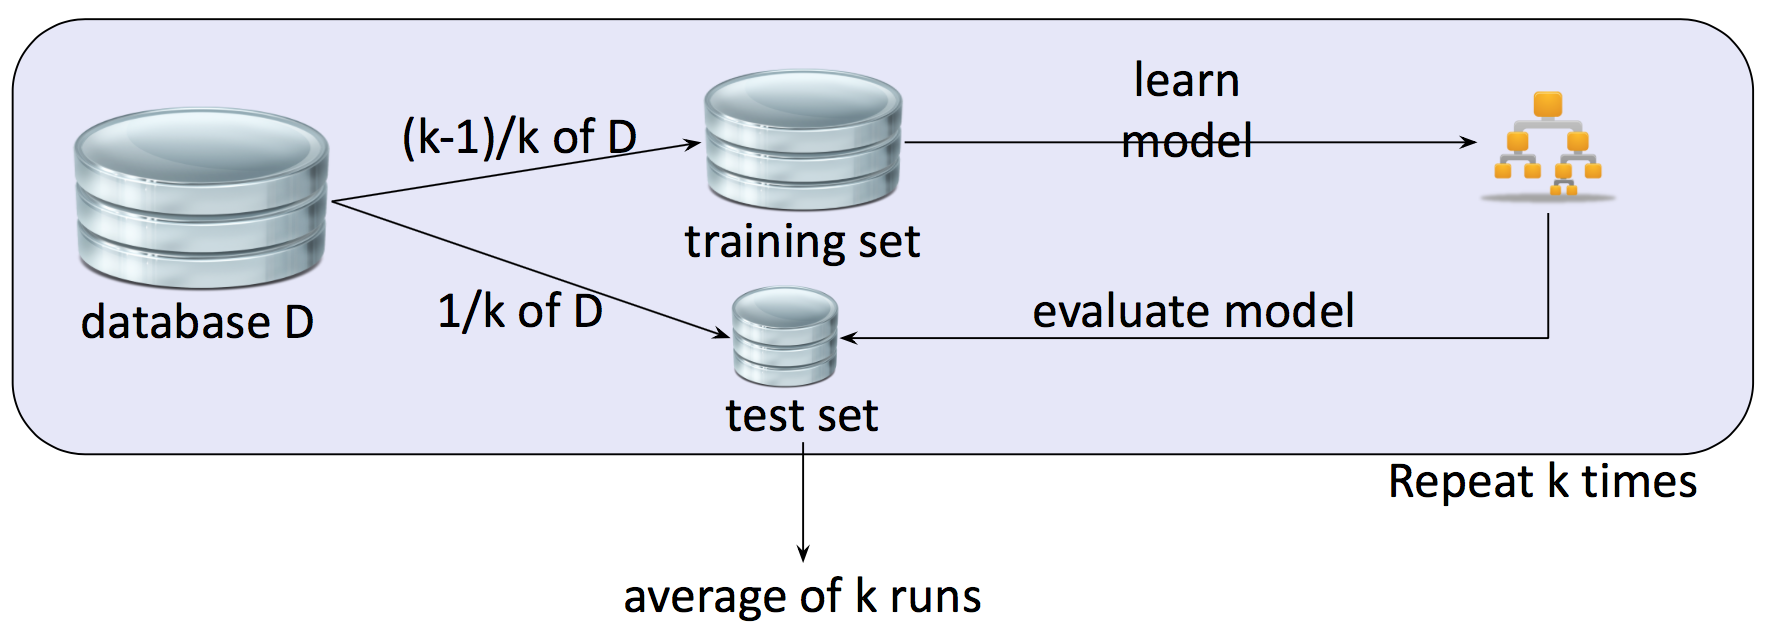
\includegraphics[width=13cm]{./img/08/kfold}
 \caption{\label{pic:kfold} \emph{K-fold} cross validation.}
\end{figure}

\end{itemize}

The bias and the variance of the model are other to important factors to take into account to select the model. In particular, they can be assessed by comparing the error metric on the training set and the test set, hence plotting the learning curves. In the ideal case, we want low bias (small training error) and low variance (small test error).

The other cases:
\begin{itemize}
\item \emph{High bias - High variance}: is the worst case and having more data does not help

\item \emph{High variance - Low Bias} it turns out in overfitting, the training error is low, the test error high though. We can opt for reducing the complexity of the model, adding regularization parameter and more data may help

\item \emph{High bias - Low Variance}: in this case we have a high-training error and high test error, we fall in underfitting. A solution could be increasing the complexity of the model (adding more features), reducing the regularization parameter.
\end{itemize}

\begin{figure}[H]%---------------FIG--------------
 \centering
 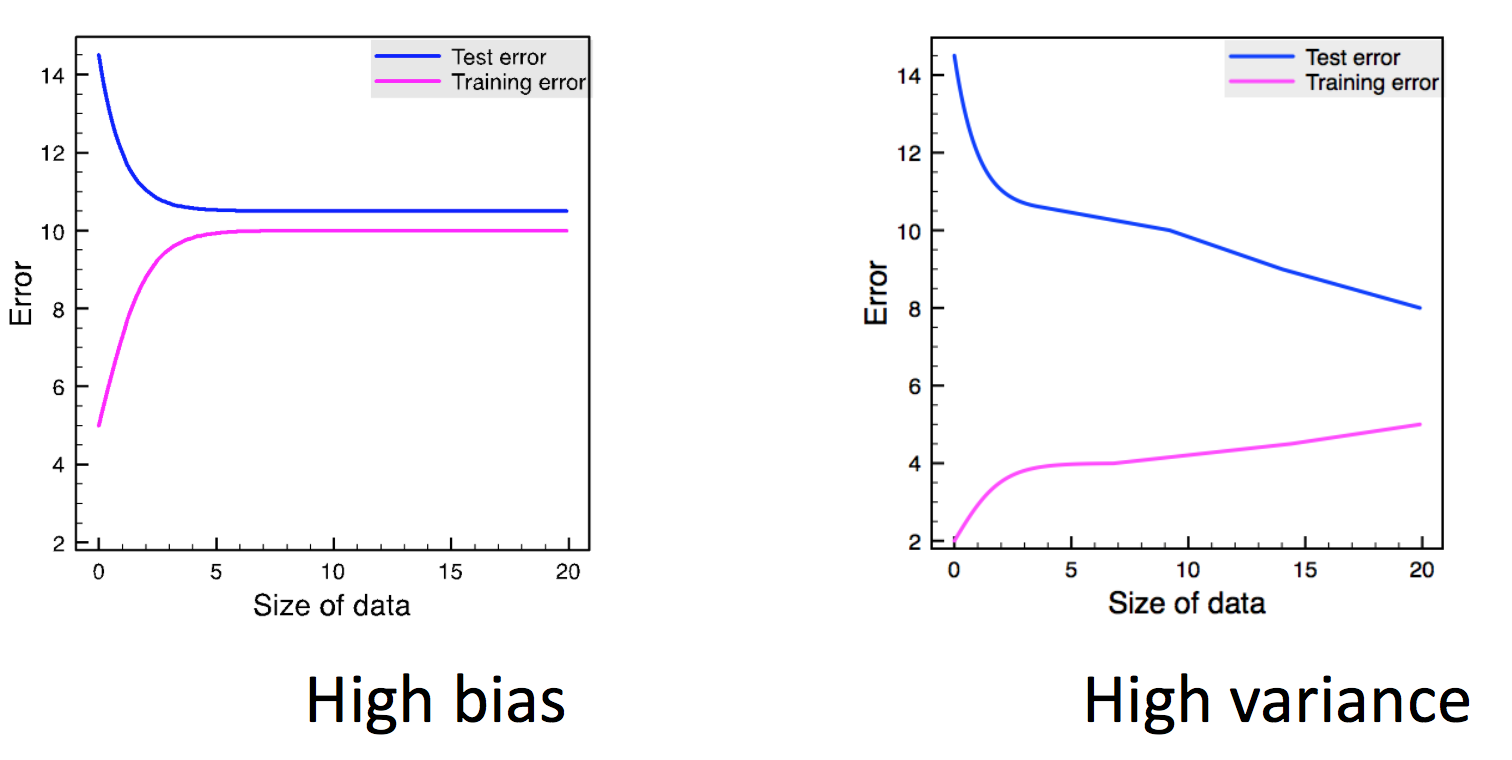
\includegraphics[width=13cm]{./img/08/bias_variance}
 \caption{\label{pic:bias_variance} \emph{Bias-Variance}: when bias is high (\emph{underfitting}), more data does not help. When variance is high (\emph{overfitting}), more data may help.
.}
\end{figure}

\subsection{Model assessment}

Model assessment is the goal of estimating the classification accuracy of a fixed model (i.e., the best model found during model selection).

At this point, to evaluate the model we use all the data set and we repeat the following steps:
\begin{enumerate}
\item \emph{Training and test}
\item \emph{Leave-one-out} or {K-fold cross-validation}
\end{enumerate}

This is a different goal than model selection. The performance obtained during model selection is a biased estimate of the true performance.